\documentclass[12pt,a4paper]{article}
\usepackage[ngerman]{babel}
\usepackage[utf8]{inputenc}
\usepackage[unicode=true,bookmarks=false,bookmarksopen=true]{hyperref}

\usepackage{xcolor}
\usepackage{graphicx}
\usepackage{tikz}

\def\checkmark{\tikz\fill[scale=0.4](0,.35) -- (.25,0) -- (1,.7) -- (.25,.15) -- cycle;}

\title{ORES Preparation IV}
\author{Tom Gülenman}
\begin{document}
\maketitle
\textit{Disclaimer: No guarantee for the correctness of information / explanations / sources is given.}\\
%
\section*{Goals}
\begin{enumerate}
\item Adjust crucial metrics list \begin{itemize}
\item to match the damaging model metrics \checkmark
\item add 2 last metrics
\end{itemize}
\item Check out mail attachments
\item Check out new Confluence pages and goals
\item Research
\begin{itemize}
\item Check out FAT Conference Docs
\item In what other cases than confusion matrices are those parameters explained?
\item Are there already visualizations of some of these parameters in any contexts?
\item Are there any applications, where I can filter for these parameters $\rightarrow$ visualizations or just about anything?
\end{itemize}
\end{enumerate}
%
\newpage
\section{Crucial metrics: \textbf{damaging}-model}
Metrics simple list:\\

\begin{tabular}{| l | l |}
\hline 
!f1 & \checkmark \\ \hline
!precision & \checkmark \\ \hline
!recall & \checkmark \\ \hline
accuracy & \checkmark \\ \hline
counts & \\ \hline
f1 & \checkmark \\ \hline
filter\_rate & \checkmark \\ \hline
fpr & \checkmark \\ \hline
match\_rate & \checkmark \\ \hline
pr\_auc & \checkmark \\ \hline 
precision & \checkmark\\ \hline
rates & \\ \hline 
recall &  \checkmark\\ \hline
roc\_auc & \checkmark \\ \hline
\end{tabular}

\begin{description}
\item The metrics are the same for the damaging and itemquality models, but a few changes will be made to the explanatory parts nontheless (compared to the version in oresDoc3). Also the structure of explanations will be changed to the following:
\item For each metric (if possible) there will be:
\begin{enumerate}
\item An intuitive explanation
\item The formula based on the \textbf{confusion matrix}
\item Its meaning based on the ``\textbf{confusion circle}''
\item Its meaning based on the \textbf{loan threshold} representation by Google (\href{https://research.google.com/bigpicture/attacking-discrimination-in-ml/}{Link})
\end{enumerate}
\end{description}
\subsection*{Explanations: References}
\begin{itemize}
\item Confusion Matrix 
\begin{description}
\item 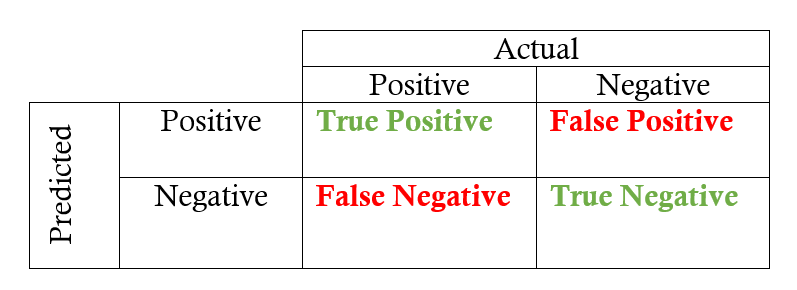
\includegraphics[scale=0.3]{resources/3/confusionMatrix}
\end{description}
\item ``Confusion Circle''
\begin{description}
\item \includegraphics[scale=0.35]{resources/3/confusionCircle}
\end{description}
\item Loan Threshold
\begin{description}
\item 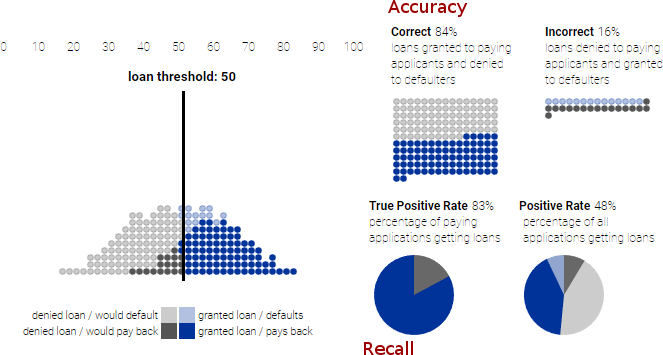
\includegraphics[scale=0.57]{resources/4/loanML4}
\end{description}
\end{itemize}
%
\subsection{recall}
\begin{enumerate}
\item Recall ($\equiv$ True Positive Rate) is defined as the ability of a model to find all relevant cases within the dataset.
\end{enumerate}
\begin{tabular}{|l|l|l|l|}
\hline
2. & 3. & 4.\\ 
$= \frac{\texttt{TP}}{\texttt{TP} + \texttt{FN}}$ & $= \frac{
\includegraphics[scale=0.1]{resources/3/confusionCircleTP}}{
\includegraphics[scale=0.1]{resources/3/confusionCircleTP+FN}}$ & $= \frac{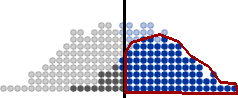
\includegraphics[scale=0.6]{resources/4/loanTP}}{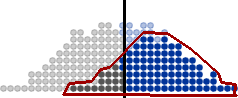
\includegraphics[scale=0.6]{resources/4/loanTP+FN}}$\\ \hline
\end{tabular}
%
\subsection{precision}
\begin{enumerate}
\item Ability of the model to find only relevant cases within the dataset
\end{enumerate}
\begin{tabular}{|l|l|l|l|}
\hline
2. & 3. & 4.\\ 
$= \frac{\texttt{TP}}{\texttt{TP} + \texttt{FP}}$ & $= \frac{
\includegraphics[scale=0.1]{resources/3/confusionCircleTP}}{
\includegraphics[scale=0.1]{resources/3/confusionCircleTP+FP}}$ & $= \frac{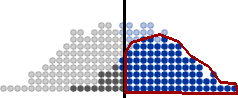
\includegraphics[scale=0.6]{resources/4/loanTP}}{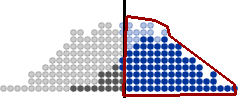
\includegraphics[scale=0.6]{resources/4/loanTP+FP}}$\\ \hline
\end{tabular}
%
\subsection{f1}
\begin{enumerate}
\item F1-Score, the harmonic mean of recall and precision, a metric from 0 (worst) to 1 (best), used to evaluate the accuracy of a model by taking recall and precision into account 
\end{enumerate}
\begin{tabular}{|l|l|l|l|}
\hline
2. & 3. & 4.\\ 
- & - & - \\ \hline
\end{tabular}
\begin{description}
\item $=2*\frac{\texttt{precision} * \texttt{recall}}{\texttt{precision}+\texttt{recall}}$
\item Compared to the simple average (of recall and precision), the harmonic mean punishes extreme values (e.g. precision 1.0 and recall 0.0 $\rightarrow$ average 0.5, but F1 $= 0$)
\end{description}
%
\subsection{fpr}
\begin{enumerate}
\item The false positive rate (\textbf{FPR}) is the probability of a false alarm
\end{enumerate}
\begin{tabular}{|l|l|l|l|}
\hline
2. & 3. & 4.\\ 
$= \frac{\texttt{FP}}{\texttt{FP} + \texttt{TN}}$ & $= \frac{
\includegraphics[scale=0.1]{resources/3/confusionCircleFP}}{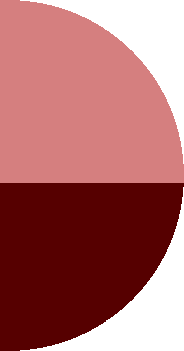
\includegraphics[scale=0.1]{resources/3/confusionCircleTN+FP}}$ & $= \frac{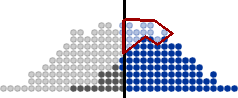
\includegraphics[scale=0.6]{resources/4/loanFP}}{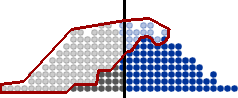
\includegraphics[scale=0.6]{resources/4/loanTN+FP}}$\\ \hline
\end{tabular}
\subsection{roc\_auc}
\begin{enumerate}
\item The \textbf{area under} the \textbf{curve} of the \textbf{ROC}-curve, a measure between 0.5 (worthless) and 1.0 (perfect: getting no FPs), rates the ability of a model to achieve a blend of recall and precision
\end{enumerate}
\begin{tabular}{|l|l|l|l|}
\hline
2. & 3. & 4.\\ 
- & -& - \\ \hline
\end{tabular}
\begin{description}
\item The receiver operating characteristic (ROC) curve plots the TPR versus FPR as a function of the model’s threshold for classifying a positive
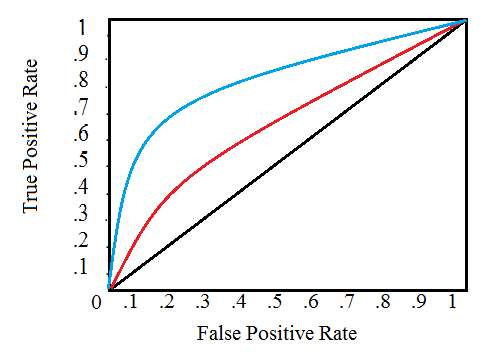
\includegraphics[scale=0.5]{resources/3/ROCcurve}
\item Increasing the threshold $\rightarrow$ moving up a curve ($\equiv$ model) to the top right corner, where all data is predicted as positive (threshold = 1.0) and vice versa
\end{description}
%
\subsection{pr\_auc}
(see: \href{http://www.chioka.in/differences-between-roc-auc-and-pr-auc/}{link 1} and \href{https://acutecaretesting.org/en/articles/precision-recall-curves-what-are-they-and-how-are-they-used}{link 2})
\begin{enumerate}
\item The \textbf{area under} the \textbf{curve} of the \textbf{PR}-curve, same: similar objective as the \textbf{roc\_auc}, but PR curves are better than ROC curves if the populations are imbalanced
\end{enumerate}
\begin{description}
\item The PR-curve plots the Precision versus the Recall 
\item 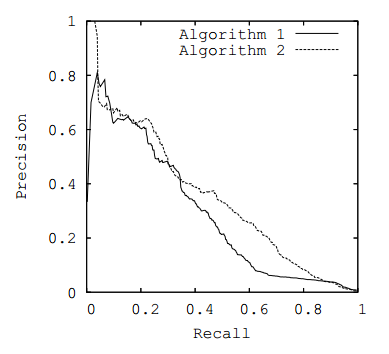
\includegraphics[scale=0.7]{resources/3/PRcurve}
\item Instead of the top left corner for the ROC-curve, here, we want to be in the top right corner for our classifier to be perfect
\end{description}
%
\subsection{accuracy}
\begin{enumerate}
\item Measuring the portion of correctly predicted data
\end{enumerate}
\begin{tabular}{|l|l|l|l|}
\hline
2. & 3. & 4.\\ 
$= \frac{\texttt{TP}+\texttt{TN}}{\texttt{Total}}$ & $= \frac{
\includegraphics[scale=0.1]{resources/3/confusionCircleTP+TN}}{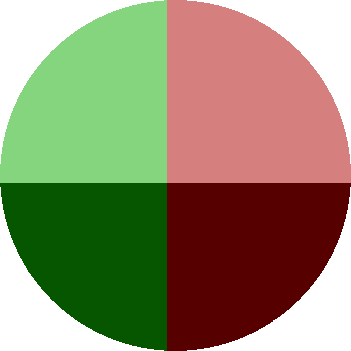
\includegraphics[scale=0.1]{resources/3/confusionCircleTotal}}$ & $= \frac{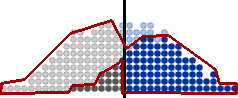
\includegraphics[scale=0.6]{resources/4/loanTP+TN}}{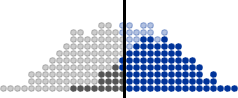
\includegraphics[scale=0.6]{resources/4/loanTotal}}$\\ \hline
\end{tabular}
\subsection{match\_rate}
\begin{enumerate}
\item The proportion of observations matched/not-matched
\end{enumerate}
\begin{tabular}{|l|l|l|l|}
\hline
2. & 3. & 4.\\ 
$= \frac{\texttt{TP}+\texttt{FP}}{\texttt{Total}}$ & $= \frac{
\includegraphics[scale=0.1]{resources/3/confusionCircleTP+FP}}{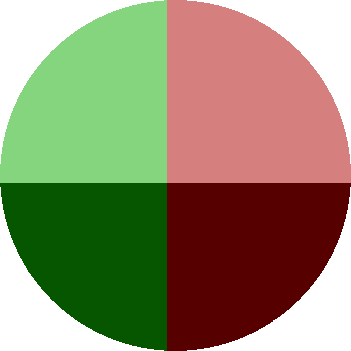
\includegraphics[scale=0.1]{resources/3/confusionCircleTotal}}$ & $= \frac{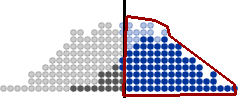
\includegraphics[scale=0.6]{resources/4/loanTP+FP}}{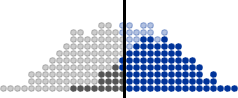
\includegraphics[scale=0.6]{resources/4/loanTotal}}$\\ \hline
\end{tabular}
%
\subsection{filter\_rate}
\begin{enumerate}
\item The proportion of observations filtered/not-filtered
\end{enumerate}
\begin{tabular}{|l|l|l|l|}
\hline
2. & 3. & 4.\\ 
$= 1-\texttt{match\_rate} = \frac{\texttt{TN}+\texttt{FN}}{\texttt{Total}} $ & $= \frac{
\includegraphics[scale=0.1]{resources/3/confusionCircleTN+FN}}{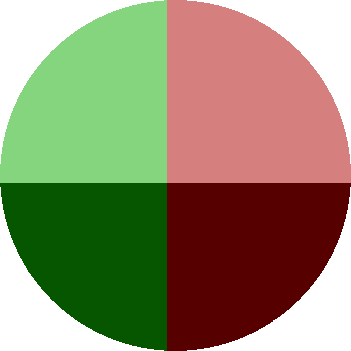
\includegraphics[scale=0.1]{resources/3/confusionCircleTotal}}$ & $= \frac{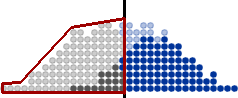
\includegraphics[scale=0.6]{resources/4/loanTN+FN}}{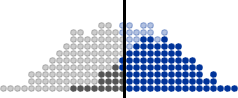
\includegraphics[scale=0.6]{resources/4/loanTotal}}$\\ \hline
\end{tabular}
%
\subsection{counts}
\begin{enumerate}
\item %TODO
\end{enumerate}
\begin{tabular}{|l|l|l|l|}
\hline
2. & 3. & 4.\\ 
 & & \\ \hline
\end{tabular}
%
\subsection{rates}
\begin{enumerate}
\item %TODO
\end{enumerate}
\begin{tabular}{|l|l|l|l|}
\hline
2. & 3. & 4.\\ 
 & & \\ \hline
\end{tabular}
%
\subsection{!$<$metric$>$}
\begin{itemize}
\item Any $<$metric$>$ with an exclamation mark is the same metric for the negative class
\item e.g. recall $= \frac{\texttt{TP}}{\texttt{TP} + \texttt{FN}} \Rightarrow$ \textbf{!}recall  $= \frac{\texttt{TN}}{\texttt{TN} + \texttt{FP}}$
\item Example usage: find all items that are not ``E'' class $\rightarrow$ look at \textbf{!}recall for ``E'' class.
\end{itemize}
\subsubsection{Existing !$<$metric$>$s}
\begin{itemize}
\item !f1
\item !precision
\item !recall
\end{itemize}
%
\subsection{Additional explanations}
\subsubsection{recall vs precision}
When increasing one of these two, the other one naturally decreases. For an intuitive example, let's take a look at \href{https://research.google.com/bigpicture/attacking-discrimination-in-ml/}{Google's Loan Threshold Simulation}:\\
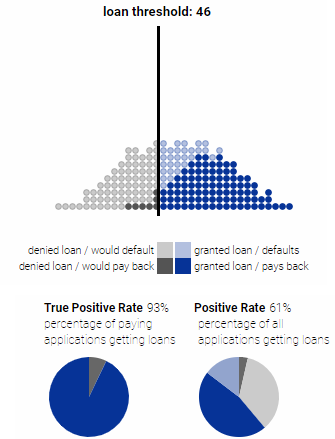
\includegraphics[scale=0.6]{resources/3/loanML3}\\
\begin{description}
\item The dark grey / dark blue dots, representing clients that would actually pay back their loan, are more and more included ($\rightarrow$ given loans) if we move the threshold further to the left.
\item But so are clients that would not. Thus moving the threshold to the left increases the \textbf{recall} (\textbf{tpr}) but decreases the \textbf{precision} and vice versa when moving to the right.
\end{description}
%
\subsubsection{roc\_auc vs pr\_auc}
see: \url{https://www.kaggle.com/general/7517}
\begin{itemize}
\item tl;dr: if the class imbalance problem exists, \textbf{pr\_auc} is more appropriate than \textbf{roc\_auc}
\begin{description}
\item If TNs are not meaningful to the problem or there are a lot more negatives than positives, \textbf{pr\_auc} is the way to go (it does not account for TNs).
\end{description}
\item In other words: 
\begin{itemize}
\item If the model needs to perform equally on the positive and negative class $\rightarrow$ \textbf{roc\_auc}
\item If it's not interesting how the model performs on negative class $\rightarrow$ \textbf{pr\_auc} (example: detecting cancer; find all positives and make sure they're correct!)
\end{itemize}
\end{itemize}
%
%
%
\newpage
\section*{Additional Information}
\begin{itemize}
\item Confluence Link (Bachelor Thesis): \url{https://intern.hcc.mi.fu-berlin.de/confluence/pages/viewpage.action?pageId=33269659}
\item Amir's mail links
\begin{itemize}
\item \href{https://www.mediawiki.org/wiki/Help:New_filters_for_edit_review/Quality_and_Intent_Filters}{New Filters for Edit Review Documentation Link}
\item \href{https://ores.wikimedia.org/v3/scores/eswiki/?models=damaging&model_info=statistics.thresholds.false.%22maximum+recall+%40+precision+%3E%3D+0.995%22%7Cstatistics.thresholds.true.%22maximum+filter_rate+%40+recall+%3E%3D+0.9%22%7Cstatistics.thresholds.true.%22maximum+recall+%40+precision+%3E%3D+0.6%22%7Cstatistics.thresholds.true.%22maximum+recall+%40+precision+%3E%3D+0.9%22&format=json}{ORES API Call Link}
\begin{description}
\item ``Basically it asks for threshold from the API when "recall is at its maximum when precision is at least 0.995"''
\end{description}
\end{itemize}
\end{itemize}
\section*{Questions}
\begin{itemize}
%
\item \colorbox{yellow}{Q:} Should I ask Aaron how he would like us to work together? I'm not sure how he meant it.
\begin{description}
\item \colorbox{orange}{A:} 
\end{description}
%
\item \colorbox{yellow}{Q:} In what situations exactly do we want to optimize the threshold in the context of user centered threshold optimization?
\begin{description}
\item \colorbox{orange}{A:} 
\end{description}
%
\item \colorbox{yellow}{Q:} VPN recommendation?
\begin{description}
\item \colorbox{orange}{A:} 
\end{description}
%
\end{itemize}
\end{document}